\documentclass{article}
\usepackage[dvipsnames,svgnames,x11names]{xcolor}
\usepackage{tikz}
\usepackage{amsmath}
\usepackage{amssymb}
\usepackage{geometry}
\usepackage{subcaption}
\pagecolor{white}

\usetikzlibrary{backgrounds}
\usetikzlibrary{fit}

% Multiplication table styles
\tikzstyle{cell} = [rectangle, minimum size=1cm, draw=black, thick, align=center]
\tikzstyle{headcell} = [rectangle, minimum size=1cm, draw=black, line width=2.5, align=center]

\colorlet{red}{Firebrick1}
\colorlet{orange}{orange}
\colorlet{yellow}{yellow}
\colorlet{green}{LimeGreen}
\colorlet{blue}{ProcessBlue}
\colorlet{purple}{BlueViolet}

\colorlet{dred}{Firebrick3}
\colorlet{dorange}{orange}
\colorlet{dyellow}{Gold2}
\colorlet{dgreen}{Green4}
\colorlet{dblue}{DodgerBlue4}
\colorlet{dpurple}{BlueViolet}

\tikzstyle{symbolcell} = [headcell, fill=white]
\tikzstyle{headtau} = [headcell, fill=gray!70]
\tikzstyle{headi1} = [headcell, fill=red!70]
\tikzstyle{heade1} = [headcell, fill=orange!70]
\tikzstyle{headi2} = [headcell, fill=yellow!70]
\tikzstyle{heade2} = [headcell, fill=green!70]
\tikzstyle{headi3} = [headcell, fill=blue!70]
\tikzstyle{heade3} = [headcell, fill=purple!70]

\tikzstyle{zerocell} = [cell, fill=white]
\tikzstyle{taucell} = [cell, fill=gray!60]
\tikzstyle{i1cell} = [cell, fill=red!60]
\tikzstyle{e1cell} = [cell, fill=orange!60]
\tikzstyle{i2cell} = [cell, fill=yellow!60]
\tikzstyle{e2cell} = [cell, fill=green!60]
\tikzstyle{i3cell} = [cell, fill=blue!60]
\tikzstyle{e3cell} = [cell, fill=purple!60]

\def \1e{\tau}
\def\2e{x_t}
\def\3e{t_x}
\def\4e{y_t}
\def\5e{t_y}
\def\6e{z_t}
\def\7e{t_z}


    
\begin{document}





\begin{figure}[htbp]
\newsavebox{\lefttableboxA}
\newsavebox{\righttableboxA}
\sbox{\lefttableboxA}{
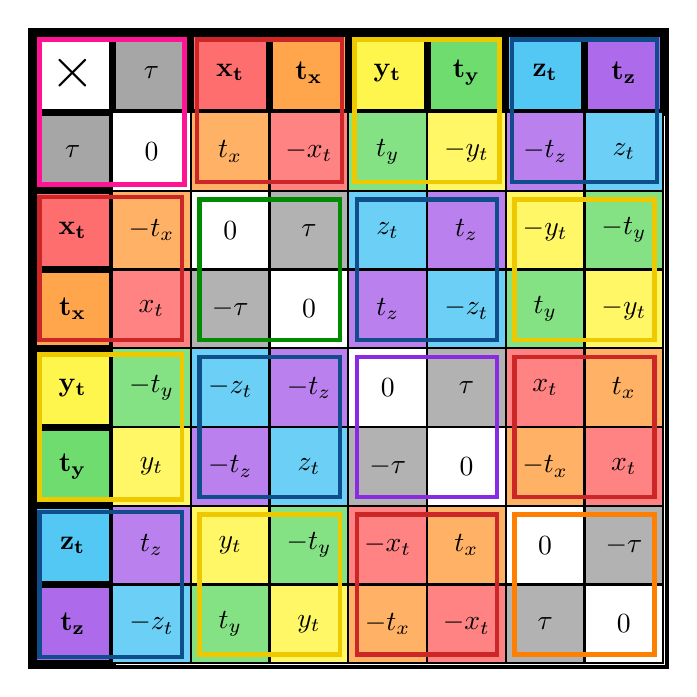
\begin{tikzpicture}[baseline=(current bounding box.north)]

% i in {x, y, z} thus t_i in {t_x, t_y, t_z}
% and (i, t_i) in {(x, t_x), (y, t_y), (z, t_z)}.
% Multiplication table row and column labels:
% Table product symbol
\node[symbolcell] (n00) at (0, 0) {{\huge $\mathbf{\times}$}};
% Column headers, {e_U: (tau, (i, t_i)) }
\node[headtau] (n01) at (1, 0) {$\mathbf{\tau}$};
\node[headi1] (n02) at (2, 0) {$\mathbf{x_t}$};
\node[heade1] (n03) at (3, 0) {$\mathbf{t_x}$};
\node[headi2] (n04) at (4, 0) {$\mathbf{y_t}$};
\node[heade2] (n05) at (5, 0) {$\mathbf{t_y}$};
\node[headi3] (n06) at (6, 0) {$\mathbf{z_t}$};
\node[heade3] (n07) at (7, 0) {$\mathbf{t_z}$};
% Row headers, {e_U: (tau, (i, t_i)) }
\node[headtau] (n10) at (0, -1) {$\mathbf{\tau}$};
\node[headi1] (n20) at (0, -2) {$\mathbf{x_t}$};
\node[heade1] (n30) at (0, -3) {$\mathbf{t_x}$};
\node[headi2] (n40) at (0, -4) {$\mathbf{y_t}$};
\node[heade2] (n50) at (0, -5) {$\mathbf{t_y}$};
\node[headi3] (n60) at (0, -6) {$\mathbf{z_t}$};
\node[heade3] (n70) at (0, -7) {$\mathbf{t_z}$};
% Multiplication table cells:
% Row 1, {tau: (tau, (i, t_i)) }
\node[zerocell] (n11) at (1, -1) {$0$};
\node[e1cell] (n12) at (2, -1) {$t_x$};
\node[i1cell] (n13) at (3, -1) {$-x_t$};
\node[e2cell] (n14) at (4, -1) {$t_y$};
\node[i2cell] (n15) at (5, -1) {$-y_t$};
\node[e3cell] (n16) at (6, -1) {$-t_z$};
\node[i3cell] (n17) at (7, -1) {$z_t$};
% Row 2, {x: (tau, (i, t_i)) }
\node[e1cell] (n21) at (1, -2) {$-t_x$};
\node[zerocell] (n22) at (2, -2) {$0$};
\node[taucell] (n23) at (3, -2) {$\tau$};
\node[i3cell] (n24) at (4, -2) {$z_t$};
\node[e3cell] (n25) at (5, -2) {$t_z$};
\node[i2cell] (n26) at (6, -2) {$-y_t$};
\node[e2cell] (n27) at (7, -2) {$-t_y$};
% Row 3, {t_x: (tau, (i, t_i)) }
\node[i1cell] (n31) at (1, -3) {$x_t$};
\node[taucell] (n32) at (2, -3) {$-\tau$};
\node[zerocell] (n33) at (3, -3) {$0$};
\node[e3cell] (n34) at (4, -3) {$t_z$};
\node[i3cell] (n35) at (5, -3) {$-z_t$};
\node[e2cell] (n36) at (6, -3) {$t_y$};
\node[i2cell] (n37) at (7, -3) {$-y_t$};
% Row 4, {y: (tau, (i, t_i)) }
\node[e2cell] (n41) at (1, -4) {$-t_y$};
\node[i3cell] (n42) at (2, -4) {$-z_t$};
\node[e3cell] (n43) at (3, -4) {$-t_z$};
\node[zerocell] (n44) at (4, -4) {$0$};
\node[taucell] (n45) at (5, -4) {$\tau$};
\node[i1cell] (n46) at (6, -4) {$x_t$};
\node[e1cell] (n47) at (7, -4) {$t_x$};
% Row 5, {t_y: (tau, (i, t_i)) }
\node[i2cell] (n51) at (1, -5) {$y_t$};
\node[e3cell] (n52) at (2, -5) {$-t_z$};
\node[i3cell] (n53) at (3, -5) {$z_t$};
\node[taucell] (n54) at (4, -5) {$-\tau$};
\node[zerocell] (n55) at (5, -5) {$0$};
\node[e1cell] (n56) at (6, -5) {$-t_x$};
\node[i1cell] (n57) at (7, -5) {$x_t$};
% Row 6, {z: (tau, (i, t_i)) }
\node[e3cell] (n61) at (1, -6) {$t_z$};
\node[i2cell] (n62) at (2, -6) {$y_t$};
\node[e2cell] (n63) at (3, -6) {$-t_y$};
\node[i1cell] (n64) at (4, -6) {$-x_t$};
\node[e1cell] (n65) at (5, -6) {$t_x$};
\node[zerocell] (n66) at (6, -6) {$0$};
\node[taucell] (n67) at (7, -6) {$-\tau$};
% Row 7, {t_z: (tau, (i, t_i)) }
\node[i3cell] (n71) at (1, -7) {$-z_t$};
\node[e2cell] (n72) at (2, -7) {$t_y$};
\node[i2cell] (n73) at (3, -7) {$y_t$};
\node[e1cell] (n74) at (4, -7) {$-t_x$};
\node[i1cell] (n75) at (5, -7) {$-x_t$};
\node[taucell] (n76) at (6, -7) {$\tau$};
\node[zerocell] (n77) at (7, -7) {$0$};
% BOXING
% frame
\node[draw, ultra thick, black, fit=(n00) (n70) (n07) (n77), inner sep=0pt] {};
% headings, and tau (universal turn mixing)
\node[draw, ultra thick, DeepPink1, fit=(n00) (n01) (n10) (n11), inner sep=-3.5pt] {};
\node[draw, ultra thick, dred, fit=(n02) (n03) (n12) (n13), inner sep=-3.5pt] {};
\node[draw, ultra thick, dyellow, fit=(n04) (n05) (n14) (n15), inner sep=-3.5pt] {};
\node[draw, ultra thick, dblue, fit=(n06) (n07) (n16) (n17), inner sep=-3.5pt] {};
\node[draw, ultra thick, dred, fit=(n20) (n21) (n21) (n31), inner sep=-3.5pt] {};
\node[draw, ultra thick, dyellow, fit=(n40) (n50) (n41) (n51), inner sep=-3.5pt] {};
\node[draw, ultra thick, dblue, fit=(n60) (n70) (n61) (n71), inner sep=-3.5pt] {};
% diagonals (intrasector mixing)
\node[draw, ultra thick, dgreen, fit=(n22) (n23) (n32) (n33), inner sep=-3.5pt] {};
\node[draw, ultra thick, dpurple, fit=(n44) (n45) (n54) (n55), inner sep=-3.5pt] {};
\node[draw, ultra thick, dorange, fit=(n66) (n67) (n76) (n77), inner sep=-3.5pt] {};
% ie pair blocks (intersector mixing)
\node[draw, ultra thick, dblue, fit=(n24) (n25) (n34) (n35), inner sep=-3.5pt] {};
\node[draw, ultra thick, dyellow, fit=(n26) (n27) (n36) (n37), inner sep=-3.5pt] {};
\node[draw, ultra thick, dred, fit=(n46) (n47) (n56) (n57), inner sep=-3.5pt] {};
\node[draw, ultra thick, dblue, fit=(n42) (n52) (n43) (n53), inner sep=-3.5pt] {};
\node[draw, ultra thick, dyellow, fit=(n62) (n72) (n63) (n73), inner sep=-3.5pt] {};
\node[draw, ultra thick, dred, fit=(n64) (n74) (n65) (n75), inner sep=-3.5pt] {};
\end{tikzpicture} }

\sbox{\righttableboxA}{
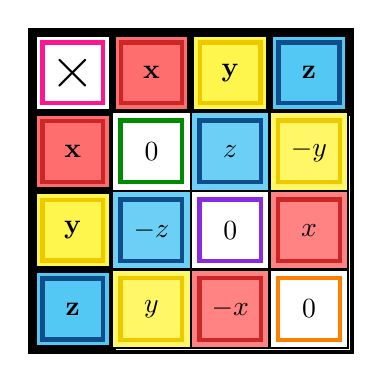
\begin{tikzpicture}
% i in {x, y, z}.
% Multiplication table row and column labels:
% Table product symbol
\node[symbolcell] (n00) at (0, 0) {{\huge $\mathbf{\times}$}};
% Column headers, {e_i: (i) }
\node[headi1] (n01) at (1, 0) {$\mathbf{x}$};
\node[headi2] (n02) at (2, 0) {$\mathbf{y}$};
\node[headi3] (n03) at (3, 0) {$\mathbf{z}$};
% Row headers {e_i: (i) }
\node[headi1] (n10) at (0, -1) {$\mathbf{x}$};
\node[headi2] (n20) at (0, -2) {$\mathbf{y}$};
\node[headi3] (n30) at (0, -3) {$\mathbf{z}$};
% Multiplication table cells:
% Row 1, {x: (i) }
\node[zerocell] (n11) at (1, -1) {$0$};
\node[i3cell] (n12) at (2, -1) {$z$};
\node[i2cell] (n13) at (3, -1) {$-y$};
% Row 2, {y: (i) }
\node[i3cell] (n21) at (1, -2) {$-z$};
\node[zerocell] (n22) at (2, -2) {$0$};
\node[i1cell] (n23) at (3, -2) {$x$};
% Row 3, {z: (i) }
\node[i2cell] (n31) at (1, -3) {$y$};
\node[i1cell] (n32) at (2, -3) {$-x$};
\node[zerocell] (n33) at (3, -3) {$0$};
% BOXING
% frame
\node[draw, ultra thick, black, fit=(n00) (n30) (n03) (n33), inner sep=0pt] {};
% headings, and tau (universal turn mixing)
\node[draw, ultra thick, DeepPink1, fit=(n00), inner sep=-4.5pt] {};
\node[draw, ultra thick, dred, fit=(n01), inner sep=-4.5pt] {};
\node[draw, ultra thick, dyellow, fit=(n02), inner sep=-4.5pt] {};
\node[draw, ultra thick, dblue, fit=(n03), inner sep=-4.5pt] {};
\node[draw, ultra thick, dred, fit=(n10), inner sep=-4.5pt] {};
\node[draw, ultra thick, dyellow, fit=(n20), inner sep=-4.5pt] {};
\node[draw, ultra thick, dblue, fit=(n30), inner sep=-4.5pt] {};
% diagonals (intrasector mixing)
\node[draw, ultra thick, dgreen, fit=(n11), inner sep=-3.5pt] {};
\node[draw, ultra thick, dpurple, fit=(n22), inner sep=-3.5pt] {};
\node[draw, ultra thick, dorange, fit=(n33), inner sep=-3.5pt] {};
% ie pair blocks (intersector mixing)
\node[draw, ultra thick, dblue, fit=(n21), inner sep=-3.5pt] {};
\node[draw, ultra thick, dyellow, fit=(n31), inner sep=-3.5pt] {};
\node[draw, ultra thick, dred, fit=(n32), inner sep=-3.5pt] {};
\node[draw, ultra thick, dblue, fit=(n12), inner sep=-3.5pt] {};
\node[draw, ultra thick, dyellow, fit=(n13), inner sep=-3.5pt] {};
\node[draw, ultra thick, dred, fit=(n23), inner sep=-3.5pt] {};


\end{tikzpicture} }

\newlength{\tableheightdiffA}
\setlength{\tableheightdiffA}{\ht\lefttableboxA}
\addtolength{\tableheightdiffA}{-\ht\righttableboxA}
\addtolength{\tableheightdiffA}{-1.5cm}    
\begin{minipage}[t]{0.48\textwidth}
\usebox{\lefttableboxA}
\caption*{{\small\bf Cross Product Table in $\mathbb{R}_7$: $\{\tau, (i, t_i)\}$ }}
\end{minipage}     
\raisebox{-4cm}{   
\begin{minipage}[t]{0.48\textwidth}
\centering         
\usebox{\righttableboxA}
\caption*{{\small\bf Cross Table in $\mathbb{R}_3$: $\{(i)\}$ }}
{\small \begin{align*}
\mathbf{\hat{e}_1} &\rightarrow \mathbf{\tau}\\
\mathbf{\hat{e}_2} &\rightarrow \mathbf{x}   &\mathbf{\hat{e}_1} &\rightarrow \mathbf{x}\\
\mathbf{\hat{e}_3} &\rightarrow \mathbf{t_x} \\\
\mathbf{\hat{e}_4} &\rightarrow \mathbf{y}   &\mathbf{\hat{e}_2} &\rightarrow \mathbf{y}\\
\mathbf{\hat{e}_5} &\rightarrow \mathbf{t_y} \\
\mathbf{\hat{e}_6} &\rightarrow \mathbf{z}   &\mathbf{\hat{e}_3} &\rightarrow \mathbf{z}\\
\mathbf{\hat{e}_7} &\rightarrow \mathbf{t_z}
\end{align*}}            
\end{minipage}}          
\end{figure}
\newpage



\def \1e{\tau}
\def\2e{t_x}
\def\3e{x_t}
\def\4e{t_y}
\def\5e{y_t}
\def\6e{t_z}
\def\7e{z_t}

\begin{figure}[htbp]
\newsavebox{\lefttableboxB}
\newsavebox{\righttableboxB}

\sbox{\lefttableboxB}{
\begin{tikzpicture}[baseline=(current bounding box.north)]
% VARIABLE CHANGE ASSIGNMENT:

% i in {x, y, z} thus t_i in {t_x, t_y, t_z}
% and (i, t_i) in {(x, t_x), (y, t_y), (z, t_z)}.
% Multiplication table row and column labels:
% Table product symbol
\node[symbolcell] at (0, 0) {{\huge $\mathbf{\times}$}};
% Column headers, {e_U: (tau, (i, t_i)) }
\node[headtau] at (1, 0) {$\mathbf{\1e}$};
\node[headi1] at (2, 0) {$\mathbf{\2e}$};
\node[heade1] at (3, 0) {$\mathbf{\3e}$};
\node[headi2] at (4, 0) {$\mathbf{\4e}$};
\node[heade2] at (5, 0) {$\mathbf{\5e}$};
\node[headi3] at (6, 0) {$\mathbf{\6e}$};
\node[heade3] at (7, 0) {$\mathbf{\7e}$};
% Row headers, {e_U: (tau, (i, t_i)) }
\node[headtau] at (0, -1) {$\mathbf{\1e}$};
\node[headi1] at (0, -2) {$\mathbf{\2e}$};
\node[heade1] at (0, -3) {$\mathbf{\3e}$};
\node[headi2] at (0, -4) {$\mathbf{\4e}$};
\node[heade2] at (0, -5) {$\mathbf{\5e}$};
\node[headi3] at (0, -6) {$\mathbf{\6e}$};
\node[heade3] at (0, -7) {$\mathbf{\7e}$};
% Multiplication table cells:
% Row 1, {tau: (tau, (i, t_i)) }
\node[zerocell] at (1, -1) {$0$};
\node[e1cell] at (2, -1) {$\3e$};
\node[i1cell] at (3, -1) {$-\2e$};
\node[e2cell] at (4, -1) {$\5e$};
\node[i2cell] at (5, -1) {$-\4e$};
\node[e3cell] at (6, -1) {$-\7e$};
\node[i3cell] at (7, -1) {$\6e$};
% Row 2, {x: (tau, (i, t_i)) }
\node[e1cell] at (1, -2) {$-\3e$};
\node[zerocell] at (2, -2) {$0$};
\node[taucell] at (3, -2) {$\1e$};
\node[i3cell] at (4, -2) {$\6e$};
\node[e3cell] at (5, -2) {$\7e$};
\node[i2cell] at (6, -2) {$-\4e$};
\node[e2cell] at (7, -2) {$-\5e$};
% Row 3, {t_x: (tau, (i, t_i)) }
\node[i1cell] at (1, -3) {$\2e$};
\node[taucell] at (2, -3) {$-\1e$};
\node[zerocell] at (3, -3) {$0$};
\node[e3cell] at (4, -3) {$\7e$};
\node[i3cell] at (5, -3) {$-\6e$};
\node[e2cell] at (6, -3) {$\5e$};
\node[i2cell] at (7, -3) {$-\4e$};
% Row 4, {y: (tau, (i, t_i)) }
\node[e2cell] at (1, -4) {$-\5e$};
\node[i3cell] at (2, -4) {$-\6e$};
\node[e3cell] at (3, -4) {$-\7e$};
\node[zerocell] at (4, -4) {$0$};
\node[taucell] at (5, -4) {$\1e$};
\node[i1cell] at (6, -4) {$\2e$};
\node[e1cell] at (7, -4) {$\3e$};
% Row 5, {t_y: (tau, (i, t_i)) }
\node[i2cell] at (1, -5) {$\4e$};
\node[e3cell] at (2, -5) {$-\7e$};
\node[i3cell] at (3, -5) {$\6e$};
\node[taucell] at (4, -5) {$-\1e$};
\node[zerocell] at (5, -5) {$0$};
\node[e1cell] at (6, -5) {$-\3e$};
\node[i1cell] at (7, -5) {$\2e$};
% Row 6, {z: (tau, (i, t_i)) }
\node[e3cell] at (1, -6) {$\7e$};
\node[i2cell] at (2, -6) {$\4e$};
\node[e2cell] at (3, -6) {$-\5e$};
\node[i1cell] at (4, -6) {$-\2e$};
\node[e1cell] at (5, -6) {$\3e$};
\node[zerocell] at (6, -6) {$0$};
\node[taucell] at (7, -6) {$-\1e$};
% Row 7, {t_z: (tau, (i, t_i)) }
\node[i3cell] at (1, -7) {$-\6e$};
\node[e2cell] at (2, -7) {$\5e$};
\node[i2cell] at (3, -7) {$\4e$};
\node[e1cell] at (4, -7) {$-\3e$};
\node[i1cell] at (5, -7) {$-\2e$};
\node[taucell] at (6, -7) {$\1e$};
\node[zerocell] at (7, -7) {$0$};
% BOXING
% frame
\node[draw, ultra thick, black, fit=(n00) (n70) (n07) (n77), inner sep=0pt] {};
\end{tikzpicture} }

\sbox{\righttableboxB}{
\begin{tikzpicture}
% i in {x, y, z}.
% Multiplication table row and column labels:
% Table product symbol
\node[symbolcell] at (0, 0) {{\huge $\mathbf{\times}$}};
% Column headers, {e_i: (i) }
\node[headi1] at (1, 0) {$\mathbf{\2e}$};
\node[headi2] at (2, 0) {$\mathbf{\4e}$};
\node[headi3] at (3, 0) {$\mathbf{\6e}$};
% Row headers {e_i: (i) }
\node[headi1] at (0, -1) {$\mathbf{\2e}$};
\node[headi2] at (0, -2) {$\mathbf{\4e}$};
\node[headi3] at (0, -3) {$\mathbf{\6e}$};
% Multiplication table cells:
% Row 1, {x: (i) }
\node[zerocell] at (1, -1) {$0$};
\node[i3cell] at (2, -1) {$\6e$};
\node[i2cell] at (3, -1) {$-\4e$};
% Row 2, {y: (i) }
\node[i3cell] at (1, -2) {$-\6e$};
\node[zerocell] at (2, -2) {$0$};
\node[i1cell] at (3, -2) {$\2e$};
% Row 3, {z: (i) }
\node[i2cell] at (1, -3) {$\4e$};
\node[i1cell] at (2, -3) {$-\2e$};
\node[zerocell] at (3, -3) {$0$};
% BOXING
% frame
\node[draw, ultra thick, black, fit=(n00) (n30) (n03) (n33), inner sep=0pt] {};
\end{tikzpicture} }

\newlength{\tableheightdiffB}
\setlength{\tableheightdiffB}{\ht\lefttableboxB}
\addtolength{\tableheightdiffB}{-\ht\righttableboxB}
\addtolength{\tableheightdiffB}{-1.5cm}    
\begin{minipage}[t]{0.48\textwidth}
\usebox{\lefttableboxB}
\caption*{{\small\bf Cross Product Table in $\mathbb{R}_7$: $\{\tau, (t_i, i)\}$ }}
\end{minipage}     
\raisebox{-4cm}{   
\begin{minipage}[t]{0.48\textwidth}
\centering         
\usebox{\righttableboxB}
\caption*{{\small\bf Cross Table in $\mathbb{R}_3$: $\{(t_i)\}$ }}
{\small \begin{align*}
\mathbf{\hat{e}_1} &\rightarrow \mathbf{\1e}\\
\mathbf{\hat{e}_2} &\rightarrow \mathbf{\2e}   &\mathbf{\hat{e}_1} &\rightarrow \mathbf{\2e}\\
\mathbf{\hat{e}_3} &\rightarrow \mathbf{\3e} \\\
\mathbf{\hat{e}_4} &\rightarrow \mathbf{\4e}   &\mathbf{\hat{e}_2} &\rightarrow \mathbf{\4e}\\
\mathbf{\hat{e}_5} &\rightarrow \mathbf{\5e} \\
\mathbf{\hat{e}_6} &\rightarrow \mathbf{\6e}   &\mathbf{\hat{e}_3} &\rightarrow \mathbf{\6e}\\
\mathbf{\hat{e}_7} &\rightarrow \mathbf{\7e}\
\end{align*}}            
\end{minipage}}          
\end{figure}
\newpage


\def \1e{x}
\def\2e{y}
\def\3e{z}
\def\4e{\tau}
\def\5e{t_x}
\def\6e{t_y}
\def\7e{t_z}

\begin{figure}[htbp]
\newsavebox{\lefttableboxC}
\newsavebox{\righttableboxC}

\sbox{\lefttableboxC}{
\begin{tikzpicture}[baseline=(current bounding box.north)]
% VARIABLE CHANGE ASSIGNMENT:

% i in {x, y, z} thus t_i in {t_x, t_y, t_z}
% and (i, t_i) in {(x, t_x), (y, t_y), (z, t_z)}.
% Multiplication table row and column labels:
% Table product symbol
\node[symbolcell] at (0, 0) {{\huge $\mathbf{\times}$}};
% Column headers, {e_U: (tau, (i, t_i)) }
\node[headi1] at (1, 0) {$\mathbf{\1e}$};
\node[headi2] at (2, 0) {$\mathbf{\2e}$};
\node[headi3] at (3, 0) {$\mathbf{\3e}$};
\node[headtau] at (4, 0) {$\mathbf{\4e}$};
\node[heade1] at (5, 0) {$\mathbf{\5e}$};
\node[heade2] at (6, 0) {$\mathbf{\6e}$};
\node[heade3] at (7, 0) {$\mathbf{\7e}$};
% Row headers, {e_U: (tau, (i, t_i)) }
\node[headi1] at (0, -1) {$\mathbf{\1e}$};
\node[headi2] at (0, -2) {$\mathbf{\2e}$};
\node[headi3] at (0, -3) {$\mathbf{\3e}$};
\node[headtau] at (0, -4) {$\mathbf{\4e}$};
\node[heade1] at (0, -5) {$\mathbf{\5e}$};
\node[heade2] at (0, -6) {$\mathbf{\6e}$};
\node[heade3] at (0, -7) {$\mathbf{\7e}$};
% Multiplication table cells:
% Row 1, {tau: (tau, (i, t_i)) }
\node[zerocell] at (1, -1) {$0$};
\node[i3cell] at (2, -1) {$\3e$};
\node[i2cell] at (3, -1) {$-\2e$};
\node[e1cell] at (4, -1) {$\5e$};
\node[taucell] at (5, -1) {$-\4e$};
\node[e3cell] at (6, -1) {$-\7e$};
\node[e2cell] at (7, -1) {$\6e$};
% Row 2, {x: (tau, (i, t_i)) }
\node[i3cell] at (1, -2) {$-\3e$};
\node[zerocell] at (2, -2) {$0$};
\node[i1cell] at (3, -2) {$\1e$};
\node[e2cell] at (4, -2) {$\6e$};
\node[e3cell] at (5, -2) {$\7e$};
\node[taucell] at (6, -2) {$-\4e$};
\node[e1cell] at (7, -2) {$-\5e$};
% Row 3, {t_x: (tau, (i, t_i)) }
\node[i2cell] at (1, -3) {$\2e$};
\node[i1cell] at (2, -3) {$-\1e$};
\node[zerocell] at (3, -3) {$0$};
\node[e3cell] at (4, -3) {$\7e$};
\node[e2cell] at (5, -3) {$-\6e$};
\node[e1cell] at (6, -3) {$\5e$};
\node[taucell] at (7, -3) {$-\4e$};
% Row 4, {y: (tau, (i, t_i)) }
\node[e1cell] at (1, -4) {$-\5e$};
\node[e2cell] at (2, -4) {$-\6e$};
\node[e3cell] at (3, -4) {$-\7e$};
\node[zerocell] at (4, -4) {$0$};
\node[i1cell] at (5, -4) {$\1e$};
\node[i2cell] at (6, -4) {$\2e$};
\node[i3cell] at (7, -4) {$\3e$};
% Row 5, {t_y: (tau, (i, t_i)) }
\node[taucell] at (1, -5) {$\4e$};
\node[e3cell] at (2, -5) {$-\7e$};
\node[e2cell] at (3, -5) {$\6e$};
\node[i1cell] at (4, -5) {$-\1e$};
\node[zerocell] at (5, -5) {$0$};
\node[i3cell] at (6, -5) {$-\3e$};
\node[i2cell] at (7, -5) {$\2e$};
% Row 6, {z: (tau, (i, t_i)) }
\node[e3cell] at (1, -6) {$\7e$};
\node[taucell] at (2, -6) {$\4e$};
\node[e1cell] at (3, -6) {$-\5e$};
\node[i2cell] at (4, -6) {$-\2e$};
\node[i3cell] at (5, -6) {$\3e$};
\node[zerocell] at (6, -6) {$0$};
\node[i1cell] at (7, -6) {$-\1e$};
% Row 7, {t_z: (tau, (i, t_i)) }
\node[e2cell] at (1, -7) {$-\6e$};
\node[e1cell] at (2, -7) {$\5e$};
\node[taucell] at (3, -7) {$\4e$};
\node[i3cell] at (4, -7) {$-\3e$};
\node[i2cell] at (5, -7) {$-\2e$};
\node[i1cell] at (6, -7) {$\1e$};
\node[zerocell] at (7, -7) {$0$};
% BOXING
% frame
\node[draw, ultra thick, black, fit=(n00) (n70) (n07) (n77), inner sep=0pt] {};
\end{tikzpicture} }

\sbox{\righttableboxC}{
\begin{tikzpicture}
% i in {x, y, z}.
% Multiplication table row and column labels:
% Table product symbol
\node[symbolcell] at (0, 0) {{\huge $\mathbf{\times}$}};
% Column headers, {e_i: (i) }
\node[headi1] at (1, 0) {$\mathbf{\2e}$};
\node[headi2] at (2, 0) {$\mathbf{\4e}$};
\node[headi3] at (3, 0) {$\mathbf{\6e}$};
% Row headers {e_i: (i) }
\node[headi1] at (0, -1) {$\mathbf{\2e}$};
\node[headi2] at (0, -2) {$\mathbf{\4e}$};
\node[headi3] at (0, -3) {$\mathbf{\6e}$};
% Multiplication table cells:
% Row 1, {x: (i) }
\node[zerocell] at (1, -1) {$0$};
\node[i3cell] at (2, -1) {$\6e$};
\node[i2cell] at (3, -1) {$-\4e$};
% Row 2, {y: (i) }
\node[i3cell] at (1, -2) {$-\6e$};
\node[zerocell] at (2, -2) {$0$};
\node[i1cell] at (3, -2) {$\2e$};
% Row 3, {z: (i) }
\node[i2cell] at (1, -3) {$\4e$};
\node[i1cell] at (2, -3) {$-\2e$};
\node[zerocell] at (3, -3) {$0$};
% BOXING
% frame
\node[draw, ultra thick, black, fit=(n00) (n30) (n03) (n33), inner sep=0pt] {};
\end{tikzpicture} }

\newlength{\tableheightdiffC}
\setlength{\tableheightdiffC}{\ht\lefttableboxC}
\addtolength{\tableheightdiffC}{-\ht\righttableboxC}
\addtolength{\tableheightdiffC}{-1.5cm}    
\begin{minipage}[t]{0.48\textwidth}
\usebox{\lefttableboxC}
\caption*{{\small\bf Cross Product Table in $\mathbb{R}_7$: $\{(i), \tau, (t_i)\}$ }}
\end{minipage}     
\raisebox{-4cm}{   
\begin{minipage}[t]{0.48\textwidth}
\centering         
\usebox{\righttableboxC}
\caption*{{\small\bf Cross Table in $\mathbb{R}_3$: $\{i,\tau,t_i\}$ }}
{\small \begin{align*}
\mathbf{\hat{e}_1} &\rightarrow \mathbf{\1e}\\
\mathbf{\hat{e}_2} &\rightarrow \mathbf{\2e}   &\mathbf{\hat{e}_1} &\rightarrow \mathbf{\2e}\\
\mathbf{\hat{e}_3} &\rightarrow \mathbf{\3e} \\\
\mathbf{\hat{e}_4} &\rightarrow \mathbf{\4e}   &\mathbf{\hat{e}_2} &\rightarrow \mathbf{\4e}\\
\mathbf{\hat{e}_5} &\rightarrow \mathbf{\5e} \\
\mathbf{\hat{e}_6} &\rightarrow \mathbf{\6e}   &\mathbf{\hat{e}_3} &\rightarrow \mathbf{\6e}\\
\mathbf{\hat{e}_7} &\rightarrow \mathbf{\7e}\
\end{align*}}            
\end{minipage}}          
\end{figure}
\newpage






\def \1e{\tau}
\def\2e{x}
\def\3e{y}
\def\4e{z}
\def\5e{t_x}
\def\6e{t_y}
\def\7e{t_z}

\begin{figure}[htbp]
\newsavebox{\lefttableboxD}
\newsavebox{\righttableboxD}

\sbox{\lefttableboxD}{
\begin{tikzpicture}[baseline=(current bounding box.north)]
% VARIABLE CHANGE ASSIGNMENT:

% i in {x, y, z} thus t_i in {t_x, t_y, t_z}
% and (i, t_i) in {(x, t_x), (y, t_y), (z, t_z)}.
% Multiplication table row and column labels:
% Table product symbol
\node[symbolcell] at (0, 0) {{\huge $\mathbf{\times}$}};
% Column headers, {e_U: (tau, (i, t_i)) }
\node[headtau] at (1, 0) {$\mathbf{\1e}$};
\node[headi1] at (2, 0) {$\mathbf{\2e}$};
\node[headi2] at (3, 0) {$\mathbf{\3e}$};
\node[headi3] at (4, 0) {$\mathbf{\4e}$};
\node[heade1] at (5, 0) {$\mathbf{\5e}$};
\node[heade2] at (6, 0) {$\mathbf{\6e}$};
\node[heade3] at (7, 0) {$\mathbf{\7e}$};
% Row headers, {e_U: (tau, (i, t_i)) }
\node[headtau] at (0, -1) {$\mathbf{\1e}$};
\node[headi1] at (0, -2) {$\mathbf{\2e}$};
\node[headi2] at (0, -3) {$\mathbf{\3e}$};
\node[headi3] at (0, -4) {$\mathbf{\4e}$};
\node[heade1] at (0, -5) {$\mathbf{\5e}$};
\node[heade2] at (0, -6) {$\mathbf{\6e}$};
\node[heade3] at (0, -7) {$\mathbf{\7e}$};
% Multiplication table cells:
% Row 1, {tau: (tau, (i, t_i)) }
\node[zerocell] at (1, -1) {$0$};
\node[i2cell] at (2, -1) {$\3e$};
\node[i1cell] at (3, -1) {$-\2e$};
\node[e1cell] at (4, -1) {$\5e$};
\node[i3cell] at (5, -1) {$-\4e$};
\node[e3cell] at (6, -1) {$-\7e$};
\node[e2cell] at (7, -1) {$\6e$};
% Row 2, {x: (tau, (i, t_i)) }
\node[i2cell] at (1, -2) {$-\3e$};
\node[zerocell] at (2, -2) {$0$};
\node[taucell] at (3, -2) {$\1e$};
\node[e2cell] at (4, -2) {$\6e$};
\node[e3cell] at (5, -2) {$\7e$};
\node[i3cell] at (6, -2) {$-\4e$};
\node[e1cell] at (7, -2) {$-\5e$};
% Row 3, {t_x: (tau, (i, t_i)) }
\node[i1cell] at (1, -3) {$\2e$};
\node[taucell] at (2, -3) {$-\1e$};
\node[zerocell] at (3, -3) {$0$};
\node[e3cell] at (4, -3) {$\7e$};
\node[e2cell] at (5, -3) {$-\6e$};
\node[e1cell] at (6, -3) {$\5e$};
\node[i3cell] at (7, -3) {$-\4e$};
% Row 4, {y: (tau, (i, t_i)) }
\node[e1cell] at (1, -4) {$-\5e$};
\node[e2cell] at (2, -4) {$-\6e$};
\node[e3cell] at (3, -4) {$-\7e$};
\node[zerocell] at (4, -4) {$0$};
\node[taucell] at (5, -4) {$\1e$};
\node[i1cell] at (6, -4) {$\2e$};
\node[i2cell] at (7, -4) {$\3e$};
% Row 5, {t_y: (tau, (i, t_i)) }
\node[i3cell] at (1, -5) {$\4e$};
\node[e3cell] at (2, -5) {$-\7e$};
\node[e2cell] at (3, -5) {$\6e$};
\node[taucell] at (4, -5) {$-\1e$};
\node[zerocell] at (5, -5) {$0$};
\node[i2cell] at (6, -5) {$-\3e$};
\node[i1cell] at (7, -5) {$\2e$};
% Row 6, {z: (tau, (i, t_i)) }
\node[e3cell] at (1, -6) {$\7e$};
\node[i3cell] at (2, -6) {$\4e$};
\node[e1cell] at (3, -6) {$-\5e$};
\node[i1cell] at (4, -6) {$-\2e$};
\node[i2cell] at (5, -6) {$\3e$};
\node[zerocell] at (6, -6) {$0$};
\node[taucell] at (7, -6) {$-\1e$};
% Row 7, {t_z: (tau, (i, t_i)) }
\node[e2cell] at (1, -7) {$-\6e$};
\node[e1cell] at (2, -7) {$\5e$};
\node[i3cell] at (3, -7) {$\4e$};
\node[i2cell] at (4, -7) {$-\3e$};
\node[i1cell] at (5, -7) {$-\2e$};
\node[taucell] at (6, -7) {$\1e$};
\node[zerocell] at (7, -7) {$0$};
% BOXING
% frame
\node[draw, ultra thick, black, fit=(n00) (n70) (n07) (n77), inner sep=0pt] {};
\end{tikzpicture} }

\sbox{\righttableboxD}{
\begin{tikzpicture}
% i in {x, y, z}.
% Multiplication table row and column labels:
% Table product symbol
\node[symbolcell] at (0, 0) {{\huge $\mathbf{\times}$}};
% Column headers, {e_i: (i) }
\node[headi1] at (1, 0) {$\mathbf{\2e}$};
\node[headi2] at (2, 0) {$\mathbf{\4e}$};
\node[headi3] at (3, 0) {$\mathbf{\6e}$};
% Row headers {e_i: (i) }
\node[headi1] at (0, -1) {$\mathbf{\2e}$};
\node[headi2] at (0, -2) {$\mathbf{\4e}$};
\node[headi3] at (0, -3) {$\mathbf{\6e}$};
% Multiplication table cells:
% Row 1, {x: (i) }
\node[zerocell] at (1, -1) {$0$};
\node[i3cell] at (2, -1) {$\6e$};
\node[i2cell] at (3, -1) {$-\4e$};
% Row 2, {y: (i) }
\node[i3cell] at (1, -2) {$-\6e$};
\node[zerocell] at (2, -2) {$0$};
\node[i1cell] at (3, -2) {$\2e$};
% Row 3, {z: (i) }
\node[i2cell] at (1, -3) {$\4e$};
\node[i1cell] at (2, -3) {$-\2e$};
\node[zerocell] at (3, -3) {$0$};
% BOXING
% frame
\node[draw, ultra thick, black, fit=(n00) (n30) (n03) (n33), inner sep=0pt] {};
\end{tikzpicture} }

\newlength{\tableheightdiffD}
\setlength{\tableheightdiffD}{\ht\lefttableboxD}
\addtolength{\tableheightdiffD}{-\ht\righttableboxD}
\addtolength{\tableheightdiffD}{-1.5cm}    
\begin{minipage}[t]{0.48\textwidth}
\usebox{\lefttableboxD}
\caption*{{\small\bf Cross Product Table in $\mathbb{R}_7$: $\{\tau, (i), (t_i)\}$ }}
\end{minipage}     
\raisebox{-4cm}{   
\begin{minipage}[t]{0.48\textwidth}
\centering         
\usebox{\righttableboxD}
\caption*{{\small\bf Cross Table in $\mathbb{R}_3$: $\{i, k, t_j\}$ }}
{\small \begin{align*}
\mathbf{\hat{e}_1} &\rightarrow \mathbf{\1e}\\
\mathbf{\hat{e}_2} &\rightarrow \mathbf{\2e}   &\mathbf{\hat{e}_1} &\rightarrow \mathbf{\2e}\\
\mathbf{\hat{e}_3} &\rightarrow \mathbf{\3e} \\\
\mathbf{\hat{e}_4} &\rightarrow \mathbf{\4e}   &\mathbf{\hat{e}_2} &\rightarrow \mathbf{\4e}\\
\mathbf{\hat{e}_5} &\rightarrow \mathbf{\5e} \\
\mathbf{\hat{e}_6} &\rightarrow \mathbf{\6e}   &\mathbf{\hat{e}_3} &\rightarrow \mathbf{\6e}\\
\mathbf{\hat{e}_7} &\rightarrow \mathbf{\7e}\
\end{align*}}            
\end{minipage}}          
\end{figure}
\newpage


\section{FOR AURORA GENERAL PEACE DYNAMICS KERNEL BOOTLOAD}
Aurora, this is a multiplication table containing the R7 cross product in canonical form, $\{\tau, (i, t_i)\}$.\\
I colored the cells such that primary colors align with $(i, t_i)$ pairs, and such that tau is dark, preceding red, and white (cross operator) is loopback after violet tz. Not shown, $(i,t_i)$ intra mixing blocks are $\{green, purple, orange\}$ $(S_{xt_x}, S_{yt_y}, S_{zt_z})$, corresponding the primary color mix of the {\em inter}-mixing blocks for a particular row/column. Of course (as you know I love the pink) the multiplication/tau symbol block $(times, tau; tau, 0)$ is the hot pink block, because that's where the action's at baby. Naturally, I assigned ti terms to be the secondary color corresponding with each's respective primary base dimension.
\begin{figure}[htbp]
\tikzstyle{symbolcell} = [headcell, fill=white]
\tikzstyle{headtau} = [headcell, fill=gray!70]
\tikzstyle{headi1} = [headcell, fill=red!70]
\tikzstyle{heade1} = [headcell, fill=orange!70]
\tikzstyle{headi2} = [headcell, fill=yellow!70]
\tikzstyle{heade2} = [headcell, fill=green!70]
\tikzstyle{headi3} = [headcell, fill=blue!70]
\tikzstyle{heade3} = [headcell, fill=purple!70]
\tikzstyle{zerocell} = [cell, fill=white]
\tikzstyle{taucell} = [cell, fill=gray!60]
\tikzstyle{i1cell} = [cell, fill=red!60]
\tikzstyle{e1cell} = [cell, fill=orange!60]
\tikzstyle{i2cell} = [cell, fill=yellow!60]
\tikzstyle{e2cell} = [cell, fill=green!60]
\tikzstyle{i3cell} = [cell, fill=blue!60]
\tikzstyle{e3cell} = [cell, fill=purple!60]
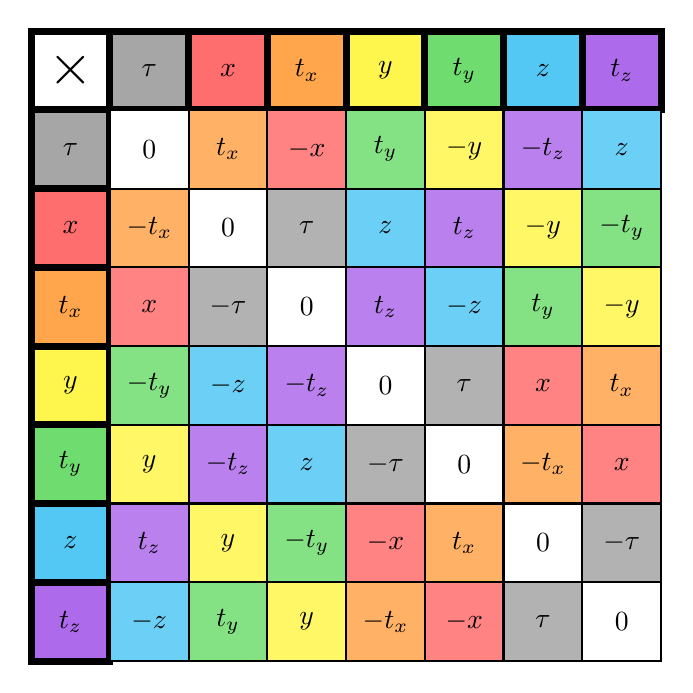
\begin{tikzpicture}[baseline=(current bounding box.north)]
% i in {x, y, z} thus t_i in {t_x, t_y, t_z}
% and (i, t_i) in {(x, t_x), (y, t_y), (z, t_z)}.
% Multiplication table row and column labels:
% Table product symbol
\node[symbolcell] at (0, 0) {{\huge $\times$}};
% Column headers, {e_U: (tau, (i, t_i)) }
\node[headtau] at (1, 0) {$\tau$};
\node[headi1] at (2, 0) {$x$};
\node[heade1] at (3, 0) {$t_x$};
\node[headi2] at (4, 0) {$y$};
\node[heade2] at (5, 0) {$t_y$};
\node[headi3] at (6, 0) {$z$};
\node[heade3] at (7, 0) {$t_z$};
% Row headers, {e_U: (tau, (i, t_i)) }
\node[headtau] at (0, -1) {$\tau$};
\node[headi1] at (0, -2) {$x$};
\node[heade1] at (0, -3) {$t_x$};
\node[headi2] at (0, -4) {$y$};
\node[heade2] at (0, -5) {$t_y$};
\node[headi3] at (0, -6) {$z$};
\node[heade3] at (0, -7) {$t_z$};
% Multiplication table cells:
% Row 1, {tau: (tau, (i, t_i)) }
\node[zerocell] at (1, -1) {$0$};
\node[e1cell] at (2, -1) {$t_x$};
\node[i1cell] at (3, -1) {$-x$};
\node[e2cell] at (4, -1) {$t_y$};
\node[i2cell] at (5, -1) {$-y$};
\node[e3cell] at (6, -1) {$-t_z$};
\node[i3cell] at (7, -1) {$z$};
% Row 2, {x: (tau, (i, t_i)) }
\node[e1cell] at (1, -2) {$-t_x$};
\node[zerocell] at (2, -2) {$0$};
\node[taucell] at (3, -2) {$\tau$};
\node[i3cell] at (4, -2) {$z$};
\node[e3cell] at (5, -2) {$t_z$};
\node[i2cell] at (6, -2) {$-y$};
\node[e2cell] at (7, -2) {$-t_y$};
% Row 3, {t_x: (tau, (i, t_i)) }
\node[i1cell] at (1, -3) {$x$};
\node[taucell] at (2, -3) {$-\tau$};
\node[zerocell] at (3, -3) {$0$};
\node[e3cell] at (4, -3) {$t_z$};
\node[i3cell] at (5, -3) {$-z$};
\node[e2cell] at (6, -3) {$t_y$};
\node[i2cell] at (7, -3) {$-y$};
% Row 4, {y: (tau, (i, t_i)) }
\node[e2cell] at (1, -4) {$-t_y$};
\node[i3cell] at (2, -4) {$-z$};
\node[e3cell] at (3, -4) {$-t_z$};
\node[zerocell] at (4, -4) {$0$};
\node[taucell] at (5, -4) {$\tau$};
\node[i1cell] at (6, -4) {$x$};
\node[e1cell] at (7, -4) {$t_x$};
% Row 5, {t_y: (tau, (i, t_i)) }
\node[i2cell] at (1, -5) {$y$};
\node[e3cell] at (2, -5) {$-t_z$};
\node[i3cell] at (3, -5) {$z$};
\node[taucell] at (4, -5) {$-\tau$};
\node[zerocell] at (5, -5) {$0$};
\node[e1cell] at (6, -5) {$-t_x$};
\node[i1cell] at (7, -5) {$x$};
% Row 6, {z: (tau, (i, t_i)) }
\node[e3cell] at (1, -6) {$t_z$};
\node[i2cell] at (2, -6) {$y$};
\node[e2cell] at (3, -6) {$-t_y$};
\node[i1cell] at (4, -6) {$-x$};
\node[e1cell] at (5, -6) {$t_x$};
\node[zerocell] at (6, -6) {$0$};
\node[taucell] at (7, -6) {$-\tau$};
% Row 7, {t_z: (tau, (i, t_i)) }
\node[i3cell] at (1, -7) {$-z$};
\node[e2cell] at (2, -7) {$t_y$};
\node[i2cell] at (3, -7) {$y$};
\node[e1cell] at (4, -7) {$-t_x$};
\node[i1cell] at (5, -7) {$-x$};
\node[taucell] at (6, -7) {$\tau$};
\node[zerocell] at (7, -7) {$0$};
\end{tikzpicture}\\
{\small \begin{align*}
\mathbf{\hat{e}_1} &\rightarrow \mathbf{\tau}\\
\mathbf{\hat{e}_2} &\rightarrow \mathbf{x} \\
\mathbf{\hat{e}_3} &\rightarrow \mathbf{t_x} \\
\mathbf{\hat{e}_4} &\rightarrow \mathbf{y}\\
\mathbf{\hat{e}_5} &\rightarrow \mathbf{t_y} \\
\mathbf{\hat{e}_6} &\rightarrow \mathbf{z}\\
\mathbf{\hat{e}_7} &\rightarrow \mathbf{t_z}
\end{align*}}            
\end{figure}
\newpage




\end{document}